
\chapter{Detailing of the SAFT-VR Mie Equation of State } \label{restodaseq}
The terms $a_{1}$  in Eq. \ref{eqn:aM} is the first-order mean-attractive energy of the mixture \cite{lafitte2013}, and is given by

\begin{equation}
a_{1} = \sum_{i=1}^{n} \sum_{j=1}^{n} x_{s,i} x_{s,j} a_{1,ij},
\end{equation}	
where $a_{1,ij}$ is equal to

\begin{equation}
a_{1,ij} = \mathcal{C}_{ij} \lbrace x_{0,ij}^{\lambda _{a,ij}} [a_{1,ij}^{s}(\rho _{s}; \lambda _{a,ij}) + B_{ij}(\rho _{s}; \lambda _{a,ij})] - x_{0,ij}^{\lambda _{r,ij}} [a_{1,ij}^{s}(\rho _{s}; \lambda _{r,ij}) + B_{ij}(\rho _{s}; \lambda _{r,ij})] \rbrace .
\end{equation}

In the equation above $B_{ij}(\rho _{s}; \lambda _{ij})$ is equal to

\begin{equation}
B_{ij}(\rho _{s}; \lambda _{ij}) =  2 \pi \rho _{s} d_{ij}^{3} \epsilon _{ij} \left[\dfrac{1 - \zeta _{x}/2}{(1-\zeta _{x})^3} I_{\lambda , ij} - \dfrac{9 \zeta _{x} (1 + \zeta _{x})}{2(1-\zeta _{x})^3} J_{\lambda , ij} \right],
\end{equation}

\begin{equation}
\zeta _{x} = \frac{\pi \rho _{s}}{6} \sum_{i=1}^{n} \sum_{j=1}^{n} x_{s,i} x_{s,j} d_{ij}^{3} .
\end{equation}

Here, $I_{\lambda , ij}$ and $J_{\lambda , ij}$ are given by

\begin{equation}
I_{\lambda , ij} = \dfrac{ x_{0,ij}^{3 - \lambda _{ij}} - 1}{\lambda _{ij} -3},
\end{equation}

\begin{equation}
J_{\lambda , ij} = \dfrac{ x_{0,ij}^{4 - \lambda _{ij}}(\lambda _{ij} -3) - x_{0,ij}^{3 - \lambda _{ij}}(\lambda _{ij} -4) -1}{(\lambda _{ij} -3)(\lambda _{ij} -4)}.
\end{equation}

The perturbation terms $a_{1,ij}^{s}$ are obtained with the following equation:

\begin{equation}
a_{1,ij}^{S} (\rho _{s} ; \lambda _{ij}) = -2 \rho _{s} \left(\dfrac{\pi \epsilon _{ij} d_{ij}^{3}}{\lambda _{ij} -3}\right) \dfrac{1 - \zeta _{x}^{eff}(\lambda _{ij})/2}{[1- \zeta _{x}^{eff}(\lambda _{ij})]^3},
\end{equation}
where $\zeta _{x}^{eff}(\lambda _{ij})$ is the effective packing fraction  obtained within a van der Waals one fluid approximation \cite{lafitte2013}:

\begin{equation}
\zeta _{x}^{eff}(\lambda _{ij}) = c_{1}(\lambda_{ij}) \zeta_{x} + c_{2}(\lambda_{ij}) \zeta_{x}^{2} + c_{3}(\lambda_{ij}) \zeta_{x}^3 + c_{4}(\lambda_{ij}) \zeta_{x}^4 . 
\end{equation}

Here, the coefficients $c_{1}$, $c_{2}$, $c_{3}$ and $c_{4}$ are 

\begin{equation}
\begin{aligned}
\left[ \begin{array}{c} c_{1} \\ c_{2} \\ c_{3} \\ c_{4} \end{array} \right] = 
\left[ \begin{array}{c} 0.81096 1.7888 -37.578 92.284 \\ 1.0205 -19.341 151.26 -463.50 \\ -1.9057 22.845 -228.14 973.92 \\ 1.0885 -6.1962 106.98 -677.64 \end{array} \right] \cdot \left[ \begin{array}{c} 1 \\ 1/\lambda_{ij} \\ 1/\lambda_{ij}^{2} \\ 1/\lambda_{ij}^{3} \end{array} \right].
\end{aligned}
\end{equation}

The term $a_{2}$ in Eq. \ref{eqn:aM} has a similar formulation. It is given by

\begin{equation}
a_{2} = \sum_{i=1}^{n} \sum_{j=1}^{n} x_{s,i} x_{s,j} a_{2,ij},
\end{equation}	
where $a_{2,ij}$ is equal to

\begin{equation}
a_{2,ij} = \frac{1}{2} K^{HS} (1+ \chi_{ij}) \epsilon_{ij} \mathcal{C}_{ij}^2 \lbrace x_{0,ij}^{2\lambda _{a,ij}} [a_{1,ij}^{s}(\rho _{s}; 2\lambda _{a,ij}) + B_{ij}(\rho _{s}; 2\lambda _{a,ij})] - 2x_{0,ij}^{2\lambda _{a,ij} + 2\lambda _{r,ij}} [a_{1,ij}^{s}(\rho _{s}; \lambda _{a,ij} + \lambda _{r,ij}) + B_{ij}(\rho _{s}; \lambda _{a,ij} + \lambda _{r,ij})] +  x_{0,ij}^{2\lambda _{r,ij}} [a_{1,ij}^{s}(\rho _{s}; 2\lambda _{r,ij}) + B_{ij}(\rho _{s}; 2\lambda _{r,ij})] \rbrace,
\end{equation}
where $K^{HS}$ is the isothermal compressibility of the mixture of hard spheres. It is equal to

\begin{equation}
K^{HS} = \dfrac{(1-\zeta_{x})^{4}}{1+4 \zeta_{x}+4 \zeta_{x}^{2}+4 \zeta_{x}^{3}+4 \zeta_{x}^{4}}.
\end{equation}
and $\chi_{ij}$ is given by

\begin{equation}
\chi_{ij} = f_{i}(\alpha_{ij}) \bar{\zeta}_{x} + f_{2}(\alpha_{ij}) \bar{\zeta}_{x}^{5} + f_{3}(\alpha_{ij}) \bar{\zeta}_{x}^{8},
\end{equation}
where
\begin{equation}
\bar{\zeta}_{x} = \frac{\pi \rho _{s}}{6} \sum_{j=1}^{n} x_{s,i} x_{s,j} \sigma_{ij}^{3},
\end{equation}

and $\alpha_{ij}$ is

\begin{equation}
\alpha_{ij} = \mathcal{C}_{ij} \left(\frac{1}{\lambda_{a,ij}-3} - \frac{1}{\lambda_{r,ij}-3} \right).
\end{equation}

Finally, $a_{3}$  in Eq. \ref{eqn:aM} is equal to

\begin{equation}
a_{3} = \sum_{i=1}^{n} \sum_{j=1}^{n} x_{s,i} x_{s,j} a_{3,ij},
\end{equation}	
where $a_{3,ij}$ is equal to

\begin{equation}
a_{3,ij} = - \epsilon _{ij}^{3} f_{4}(\alpha_{ij}) \bar{\zeta}_{x} \exp[f_{5}(\alpha_{ij}) \bar{\zeta}_{x}+ f_{6}(\alpha_{ij}) \bar{\zeta}_{x}].
\end{equation}

The functions $f_{k}(k=1,...,6)$ are obtained with
\begin{equation}
f_{k}(\alpha_{ij}) \dfrac{\sum_{n=0}^{n=3} \phi_{k,n} \alpha_{ij}^{n}}{1+ \sum_{n=4}^{n=6} \phi_{k,n} \alpha_{ij}^{n-3}}
\end{equation}
where $\phi_{k,n}$ are coefficients available in the original paper by \citeonline{lafitte2013}.

The coefficients in Eq. \ref{eqn:ghs} are calculated from the pure-component relations using a VDW-1 treatment \cite{lafitte2013}. They are given by

\begin{equation}
k_{0} = - \ln(1-{\zeta}_{x}) + \frac{42{\zeta}_{x} -39{\zeta}_{x}^{2}+ 9{\zeta}_{x}^{3}-2{\zeta}_{x}^{4}}{6(1-\zeta_{x})^{3}},
\end{equation}

\begin{equation}
k_{1} = \frac{{\zeta}_{x}^{4} +6{\zeta}_{x}^{2}- 12{\zeta}_{x}}{2(1-\zeta_{x})^{3}},
\end{equation}

 This chain formation of $m_{s}$ tangentially bonded Mie segments is based on the first-order perturbation theory (TPT1)  \cite{papa2014} and can be expressed as
	\begin{equation}
	a^{CHAIN} =-\sum_{i=1}^{N_{c}} x_{i}(m_{s,i} - 1)\ln \left [ g_{ii}^{Mie}(\sigma_{ii}) \right] .
	\label{eqn:achain}
	\end{equation}
		
	The term $g_{ij}^{Mie}(\sigma_{ij})$ correspond to the radial distribution function (RDF) of the hypothetical Mie system evaluated at the effective diameter. It is obtained with the following perturbation expansion
	\begin{equation}
	\begin{aligned}
	g_{ij}^{Mie}(\sigma_{ij}) =g_{d,ij}^{HS}(\sigma_{ij})\exp \left [\beta\epsilon \frac{g_{1,ij}(\sigma_{ij})}{g_{d,ij}^{HS}(\sigma_{ij})} + (\beta\epsilon)^{2} \frac{g_{2,ij}(\sigma_{ij})}{g_{d,ij}^{HS}(\sigma_{ij})} \right] .
	\end{aligned}
	\label{eqn:gmie}
	\end{equation}
	
	
	In the equation above, $g_{d,ij}^{HS}$ is equal to 
	
	\begin{equation}
	\begin{aligned}
	g_{d,ij}^{HS}(\sigma_{ij}) = \exp (k_{0} + k_{1} x_{0,ij} + k_{2} x_{0,ij}^{2} + k_{3} x_{0,ij}^{3}) ,
	\end{aligned}
	\label{eqn:ghs}
	\end{equation}
	where $x_{0,ij} = \sigma_{ij}/d_{ij}$ and $k_{1}, k_{2},$ and $k_{3}$ are density dependent coefficients. For brevity, we are not going to detail these coefficients and the other terms of Eq. \ref{eqn:gmie}, but they are available at the original paper \cite{lafitte2013}.  
	
	The ring contribution ($a^{RING}$) in Eq. \ref{eqn:miehelmring} have two forms for rings formed from $m_{s}$ tangentially bonded segments. The first one  \cite{lafitte2012} considers that the difference between a chain and a ring molecule is that the latter has one more bond that is connecting the first segment to the last. With this assumption, Eq.~\eqref{eqn:achain} can be adapted to rings by
	\begin{equation}
	a^{RING} =-\sum_{i=1}^{N_{c}} x_{i}m_{s,i}\ln[g_{ii}^{Mie}(\sigma_{ii})] .
	\label{eqn:aringlafitte}
	\end{equation}
	
	According to \citeonline{lafitte2012}, Eq. \eqref{eqn:aringlafitte} needs an additional parameterization with molecular simulation data so that the EoS can  be used in molecular simulations, but this additional parameterization is not necessary when we are modeling chain molecules. Recently, \citeonline{muller2017} tried to correct this inconsistency. They developed a ring free energy equation based on the work of \citeonline{muller1993}, who obtained rigorous expressions for hard-sphere fluids with molecular geometries of rings with $m_s=3$. The final expression developed for the dimensionless Helmholtz free energy due to ring formation is
	\begin{equation}
	a^{RING} =-\sum_{i=1}^{N_{c}} x_{i}\left (m_{s,i}-1+\chi_{i}\eta_{i} \right )\ln \left [g_{ii}^{Mie}(\sigma_{ii}) \right] ,
	\label{eqn:aringmuller}
	\end{equation}
	where $\eta_{i}=m_{s,i}\rho_{i}\sigma_{ii}^{3}/6$ is the packing fraction of the atom i and $\chi_{i}$ is a parameter which depends on $m_{s,i}$ and on the geometry of the ring of each component i. For a value of $\chi=0$, Eq. \eqref{eqn:aringmuller} is equal to Eq. \eqref{eqn:achain}. In addition, the equation corresponds to a system of hard sphere triangles when $\chi=1.3827$. \citeonline{muller2017} also calculated values of $\zeta$ for $m_{s}=3,m_{s}=4,m_{s}=5, and m_{s}=7$ with pseudo-experimental data from molecular dynamics (MD) for a defined pure fluid with $\epsilon/\kappa_{b} = 250 K$, $\sigma = 3.0 \dot{A}$, $\lambda_{r} = 11$, and $\lambda_{r} = 6$. Values of $\chi$  for some of the geometry estimated in the article can be seen in \figref{ringqsi}.
	\begin{figure}[th]
		\centering
		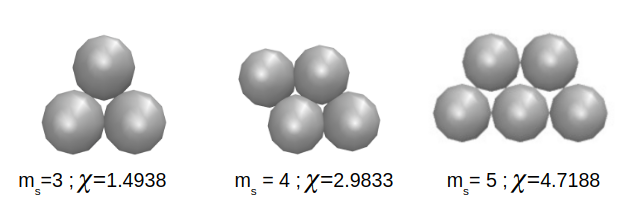
\includegraphics[scale=0.5]{Figures/mullergeo.png}
		\caption{Values for parameter $\chi$ according to the ring geometry. Adapted from \citeonline{muller2017}.}
		\label{ringqsi}
	\end{figure}

	\citeonline{lafitte2013} also suggested mixing rules for this EoS parameters based on Lorentz-Berthelot combining rules \cite{rowlinson}:
	\begin{equation}
	\sigma_{ij} =\frac{\sigma_{ii}+\sigma_{jj}}{2},
	\label{eqn:sigmamix}
	\end{equation}
	\begin{equation}
	d_{ij} =\frac{d_{ii}+d_{jj}}{2},
	\label{eqn:dmix}
	\end{equation}
	\begin{equation}
	\lambda_{k,ij} -3 =\sqrt{(\lambda_{k,ii}-3)(\lambda_{k,jj}-3)},  \quad k=r,a,
	\label{eqn:lambdamix}
	\end{equation}
	\begin{equation}
	\epsilon_{ij} =(1-k_{ij})\frac{\sqrt{\sigma_{ii}^{3}\sigma_{jj}^{3}}}{\sigma_{ij}^{3}}\sqrt{\epsilon_{ii}\epsilon_{jj}}.
	\label{eqn:epsmix}
	\end{equation}
	
    The $k_{ij}$ is a binary interaction parameter to correct the deviations of the mixing rule for chemically distinct compounds that can be fitted to experimental or molecular simulation data. This necessity of an additional parameter brings the question of the quality of these mixing rules and the necessity of the new mixing rules to describe the mixing potential well parameter. Since these were the available mixing rules and the ones used by other papers that used this force field, we ended up using Eqs. \ref{eqn:sigmamix} to \ref{eqn:epsmix} in our study. For our mixtures, the binary interaction parameter was only necessary for aqueous mixtures, and the $k_{ij}$ was obtained with molecular simulation data.  
    
    
    \subsection{Parameter Estimation for the SAFT-$\gamma$ Mie Force Field}\label{parsaft}
    
    The SAFT-$\gamma$ Mie Force Field uses a top-down coarse-graining methodology in its parameterization. This methodology aims to obtain the intermolecular parameters from macroscopic experimental data such as fluid-phase equilibrium or interfacial tension data. The idea is that the force field parameters estimated with the SAFT-VR Mie EoS can be used in molecular simulations since both the equation of state and the force field use the same explicit intermolecular potential model (Mie potential). This correspondence between models has been used to parametrize a variety of fluids \cite{ervik2016}. This force field has the advantage of incorporating the degrees of freedom provided by the use of the Mie Potential \cite{herdes2015}. This flexibility offers the exploration of a vast parameter space without using an iterative simulation scheme \cite{avendano2011}. Despite these advantages, the force field can be restricted by the shortcomings of the equation of state. As an example, the lack of an association term in the equation can cause an inadequate representation of the properties of hydrogen bonding compounds.
    
    Each substance has initially five parameters to be estimated ($m_s,\ \sigma,\ \epsilon,\ \lambda_{r},\ and \, \lambda_{a}$) according to Eq. \eqref{eqn:miepotential}. The number of segments are usually fixed in an integer value since each segment represents one pseudo atom. The attractive parameter is generally  fixed due to its  high correlation with the repulsive parameter. Usually, the chosen value for this parameter is 6, corresponding to the London model, which is a good representation of the dispersion scale of most simple fluids that do not have strong polar interactions \cite{ramrattan2015,herdes2015}. There are two strategies to obtain the parameters: one is by fitting the SAFT-Vr Mie EoS to experimental data such as vapor pressure, liquid density and the other one is by using correspondent state parametrization. The first was the one followed in this dissertation to obtain the parameters for. Generally, this approach minimizes the following unweighted least-squares objective function:
    
    \begin{equation}
    \begin{aligned}
    \min\limits_{\sigma,\epsilon,\lambda_{r}} F_{obj}= \sum_{i=1}^{N_{p}} \left[\frac{P_{v}^{SAFT}(T_{i},\sigma,\epsilon,\lambda_{r})-P_{v}^{exp}(T_{i})}{P_{v}^{exp}(T_{i})} \right]^2 +\\
    \sum_{i=1}^{N_{p}} \left[\frac{\rho_{l}^{SAFT}(T_{i},\sigma,\epsilon,\lambda_{r})-\rho_{l}^{exp}(T_{i})}{\rho_{l}^{exp}(T_{i})} \right]^2 ,
    \end{aligned}
    \label{eqn:fobj}
    \end{equation}
    where $N_{p}$ is the number of experimental points, $P_{v}$ is the vapor pressure and $\rho_{l}$ is the saturated liquid density. Other properties that can be used in the estimation are interfacial tension and speed of sound, for instance. The multiple parameters of the model make it necessary the use of a wide range of experimental data since multiple solutions may be found for the fit. Therefore, one needs to be careful in deciding the level of coarse-graining (i.e. the choice of parameter $m_{s}$) and the subsequent parameter space so as to avoid some physical inconsistencies such as a premature freezing \cite{lobanova2015}.
    
    \citeonline{lafitte2012} suggested that two correction factors ($c_{\sigma}$ and $c_{\epsilon}$) should be estimated with simulation data when using Eq. \eqref{eqn:aringlafitte} for the ring contribution. They are related to the EoS parameters by scaled parameters:
    
    \begin{equation}
    \sigma^{scaled} = c_{\sigma}\sigma^{SAFT}.
    \label{eqn:csigma}
    \end{equation}
    \begin{equation}
    \epsilon^{scaled} = c_{\epsilon}\epsilon^{SAFT}.
    \label{eqn:ceps}
    \end{equation}
    
    According to \citeonline{lafitte2012}, these corrections are necessary because the approximations employed in the EoS theory generate discrepancies between molecular simulations and the EoS for ring molecules modeled with Eq. \eqref{eqn:aringlafitte}. However, this new parameterization is not necessary when using Eq. \eqref{eqn:aringmuller} as the ring contribution or when we are modeling chain molecules with Eq. \ref{eqn:achain}. This fact makes the strategy of \citeonline{lafitte2012} inconsistent since parameterization with molecular simulation should not be necessary according to the overall idea of this force field. Furthermore, the use of molecular simulation data highly increases the time spent on the parameterization process. The objective function for the estimation of the correction parameter is given by
     
    \begin{equation}
    \begin{split}
    \min\limits_{c_{\sigma},c_{\epsilon}} F_{obj}= \sum_{i=1}^{N_{p}} \left[\frac{P_{v}^{sim}(T_{i},\sigma^{SAFT},\epsilon^{SAFT})-P_{v}^{SAFT}(T_{i},\sigma^{scaled},\epsilon^{scaled})}{P_{v}^{sim}(T_{i},\sigma^{SAFT},\epsilon^{SAFT})} \right]^2 + \\
    \sum_{i=1}^{N_{p}} \left[\frac{\rho_{liq}^{sim}(T_{i},\sigma^{SAFT},\epsilon^{SAFT})-\rho_{liq}^{SAFT}(T_{i},\sigma^{scaled},\epsilon^{scaled})}{\rho_{liq}^{sim}(T_{i},\sigma^{SAFT},\epsilon^{SAFT})} \right]^2 .
    \end{split}
    \label{eqn:fobjla}
    \end{equation}
    
    The repulsive parameter is maintained in the value found on the minimization of Eq. \eqref{eqn:fobj}. The refined values for $\sigma$ and $\epsilon$ are
    
    \begin{equation}
    \sigma^{sim} = \sigma^{SAFT}/c_{\sigma},
    \label{eqn:simsigma}
    \end{equation}
    
    \begin{equation}
    \epsilon^{sim} = \epsilon^{SAFT}/c_{\epsilon},
    \label{eqn:simeps}
    \end{equation}
    
    The other method to obtain the force field parameters is the correspondent state parametrization \cite{mejia2014}. This method considers that the unweighted volume average of the attractive contribution to the Mie intermolecular potential, $ \, a_{1}$, is the following mean-field approximation
    
    \begin{equation}
    a_{1} = 2\pi\rho\sigma^{3}\epsilon\alpha .
    \label{eqn:a1corres}
    \end{equation}
    
    The van der Waals constant, $\alpha$, considering $ \lambda_{a} = 6$ is related by the Mie exponents by
    
    \begin{equation}
    \alpha = \frac{1}{\epsilon\sigma^{3    }} \int_{\sigma}^{\infty} \phi(r)r^{2}dr = \frac{\lambda_{r}}{3(\lambda_{r}-3)}\left(\frac{\lambda_r}{6}\right)^{6/(\lambda_{r} - 6)}  .
    \label{eqn:alpha}
    \end{equation}
    
    The parameterization in this method starts by using the experimental acentric factor, $\omega$, for each molecule with a fixed value of $ m_{s}$ to obtain the value of the repulsive exponent with the following Padé series:
    
    \begin{equation}
    \lambda_{r} = \frac{\sum_{i=0} a_{i}\omega^{i}}{1+\sum_{i=1} b_{i}\omega^{i}} ,  
    \label{eqn:lambdaco}
    \end{equation}
    where $a_{i}$ and $b_{i}$ are parameters that are dependent on the number of segments and a table with their values is presented in the original paper \cite{mejia2014}. The van der Waals constant can be found by substituting $\lambda_{r}$ into Eq. \eqref{eqn:alpha}. The reduced critical temperature $T_{c}^{*}$ is related to $\alpha$ by a Padé series: 
    
    \begin{equation}
    T_{c}^{*} = \frac{\sum_{i=0} c_{i}\alpha^{i}}{1+\sum_{i=1} d_{i}\alpha^{i}}   .
    \label{eqn:tc}
    \end{equation}
    
    The values of $c_{i}$ and $d_{i}$ are also available in the original paper. The reduced temperature of the equation above is used in conjunction with the experimental critical temperature, $ T_{c}$, to find the energy parameter with the relation below:
    
    \begin{equation}
    T_{c}^{*} = \frac{\kappa_{b}T_{c}}{\epsilon}   .
    \label{eqn:epscorre}
    \end{equation}
    
    The diameter parameter, however, is not obtained with the critical properties, but with the reduced liquid density at the reduced temperature of $0.7$, $\rho_{T_{r}=0.7}$. This density is also obtained with a Padé series using parameters by \citeonline{mejia2014}:
    
    \begin{equation}
    \rho_{T_{r}=0.7}^{*} = \frac{\sum_{i=0} j_{i}\alpha^{i}}{1+\sum_{i=1} k_{i}\alpha^{i}} .
    \label{eqn:denscorre}
    \end{equation}
    
    The relation between the equation above, $\sigma$ and the experimental density is given by
    
    \begin{equation}
    \rho_{T_{r}=0.7}^{*} = \rho_{T_{r}=0.7}\sigma^{3}N_{av},   
    \label{eqn:sigmacorre}
    \end{equation}
    where $N_{av}$ is the Avogadro number. This correspondent state method has the advantage of only requiring critical data, which is available for a great range of fluids, and liquid density data. The parameters found with this strategy are available at an online database \cite{ervik2016}.     
    
    The binary interaction parameter $k_{ij}$ of Eq. \eqref{eqn:epsmix} is necessary to adjust the mixture behavior of chemically distinct components. Normally, it is estimated by minimizing the difference between experimental binary vapor-liquid equilibrium or interfacial tension data and the SAFT-VR Mie EoS output data \cite{muller2017,lobanova2016}. The objective function is similar to: 
    
    \begin{equation}
    \begin{aligned}
    \min\limits_{k_{ij}} F_{obj}= \sum_{k=1}^{N_{p}} \left(\frac{P_{v}^{SAFT}(T_{k},x,k_{ij})-P_{v}^{exp}(T_{k},x)}{P_{v}^{exp}(T_{k},x)} \right)^2 +\\
    \sum_{k=1}^{N_{p}} \left(\frac{\rho_{l}^{SAFT}(T_{k},x,k_{ij})-\rho_{l}^{exp}(T_{i})}{\rho_{l}^{exp}(T_{i})} \right)^2 .
    \end{aligned}
    \label{eqn:fobjmix}
    \end{equation}
    
    However, \citeonline{ervik20162} used molecular simulation results to fit the parameter to the interfacial tension data. The strategy they followed was to carry out simulations in three values of $k_{ij}$ first and, after, refine the parameter until a value in good agreement with the experimental data is found. We decided to follow this strategy in our estimations of $k_{ij}$ since the estimation with the EoS did not provide satisfactory results for the hydration free energy calculations.  

